\documentclass[a4paper,12pt]{report}

\usepackage{alltt, fancyvrb, url}
\usepackage{graphicx}
\usepackage[utf8]{inputenc}
\usepackage{float}
\usepackage{hyperref}

\usepackage[italian]{babel}

\usepackage[italian]{cleveref}

\title{\textbf{Elaborato per il corso di Basi Di Dati \\ A.A 2022/2023}}

\author{Ettore Farinelli \\ ettore.fainelli@studio.unibo.it \\ 0001019995}

\date{\today}

\begin{document}

\maketitle

\tableofcontents

\chapter{Analisi dei requisiti}
Si pone l'obbiettivo di realizzare un database capace di gestire un organizzazione di arti marziali come può essere, 
per esempio, \textsc{L'Ultimate Fighting Championship, (UFC)}. La base di dati dovrà quindi essere capace di registrare 
nuovi \textbf{lottatori} e in caso rimuoverli(squalifica, infortuneo, ritiro). Inoltre sarà possibile registrare \textbf{eventi}, 
dove i combattenti si scontreranno aggiornando (dopo gli \textbf{scontri}), gli \textbf{score} dei partecipanti 
e in caso le \textbf{classifiche}.

\section{Intervista}
A seguito di una prima intervista si sono ottenute le seguenti richieste:\medskip

Per ogni partecipante alla lega bisogna tenere traccia del nome, cognome, codice fiscale, data di nascita, team, peso e \textbf{arte 
marziale} in cui vuole lottare. Alla iscrizione di un nuovo lottatore esso verrà inserito all'ultimo 
posto nella classifica della propria categoria. Ci sarà la possibilità di registrare i \textbf{team} dei combattenti tenendo traccia di: nome, amministratore e 
origine. Saranno presenti diverse classifiche per ogni tipo di categoria dove i lottatori saranno ordinati 
in base ai loro \textbf{record} (V, P, S), dove le vittorie assegnano 3 punti, i pareggi 1 e le sconfitte 0.\par
Le categorie in cui verranno suddivisi i membri della lega sono: \textit{Peso Piuma} (fino a 65kg), \textit{Welterweight} 
(65kg - 77kg), \textit{Peso Medio} (77kg - 84kg) e \textit{Pesi Massimi} (da 84kg in poi). Inoltre non ci sarà una vera e propria 
divisione in arti marziali in quanto combattenti praticanti discipline diverse potranno scontrarsi tra loro, le arti marziali sono le 
seguanti: \textit{MMA} (Mixed Martial Arts), \textit{BJJ} (Brazial Jiu Jitsu) e infine \textit{Muay Thai}. Per ogni 
partecipante dovrà essere inserita la disciplina di competenza possibilmente modificabile in futuro (sarà gestito in maniera 
analoga il peso). Inoltre, partecipanti appartenenti a una determinata categoria potranno scontrarsi solo con altri membri 
della stessa. Gli eventi saranno constituiti da almeno 2 combattimenti ciascuno, bisognerà tener traccia del: nome dello stadio, 
luogo (nazione), costo noleggio stadio, spesa staff, data, orario inizio, orario fine, biglietti standard venduti, biglietti 
premium venduti, costo biglietti standard, costo biglietti premium, introiti netti, inoltre sarà necessario poter associare a un 
evento degli sponsor selezionabili tra quelli disponibili che hanno effettuato un contratto con la lega. Ogni lottatore partecipante 
riceverà un pagamento extra e verrà calcolata una quantità di guadagni tramite pubblicità, tutto in base al numero di biglietti 
venduti per l'evento, così da poter calcolare gli introiti dell'evento, il quale verrà aggiunto in una \textsc{History} dove saranno 
immagazzinati tutti gli eventi passati.

\section{Definizioni}
\begin{itemize}
    \item \textbf{Lottatore}: partecipante alla lega.
    \item \textbf{Organizzatore}: amministratore che ha l'accesso al database e le autorizzazioni per gestirlo. 
    \item \textbf{Evento}: un insieme di scontri avente un luogo e una data.
    \item \textbf{Scontro}: un incontro tra due lottatori della stessa categoria.
    \item \textbf{Classifica}: lista numerata in ordine dal partecipante migliore al peggiore in base ai record personali.
    \item \textbf{Arte marziale}: disciplina frequentante da un partecipante.
    \item \textbf{Team}: associazione a cui possono far parte 1 o piu combattenti, ha lo scopo di seguirli durante gli scontri e allenarli.
    \item \textbf{Record}: terna di vittorie, pareggi, sconfitte (V, P, S), ogni prtecipante ha la sua che definisce la sua posizione in 
        classifica.
\end{itemize}

\subsection{Operazioni Utente}
\begin{itemize}
    \item Visualizzare classifiche.
    \item Visualizzare news.
    \item Visualizzare eventi.
    \item Visualizzare lottatori.
\end{itemize}

\subsection{Operazioni Pubblicitario}
\begin{itemize}
    \item Scrivere news.
\end{itemize}

\subsection{Operazioni Amministratore}
\begin{itemize}
    \item Registrare un nuovo lottatore.
    \item Rimuovere un lottatore.
    \item Registrare un nuovo team.
    \item Rimuovere un team.
    \item Aggiungere/Rimuovere uno sponsor.
    \item Registrare/Rimuovere pubblicitari.
    \item Registrare un evento.
    \item Rimuovere news.
    \item Modificare i dati dei partecipanti.
\end{itemize}

\chapter{Progettazione Concettuale}
\section{Amministratore}
L'amministratore è colui che utilizza effettivamente a livello di applicazione il database, quindi sarà lui che organizzerà tutte  
le altri parti principali del database come i lottatori, gli eventi, i team e le sponsorizzazioni.

\section{Lottatore}
I lottatori sono il cuore dell'intero database, per questo parte tutto dall'entità "lottatore" a cui sarà associata un'entità 
"record" creata in modo tale da poter tener traccia dello score di ogni combattente, inoltre i lottatore potranno o meno far parte 
di un team precedentemente registrato. Infine, ogni lottatore potrà partecipare a uno scontro per ogni evento, 
in questo caso non sono riuscito a gestire (a livello di schema concettuale) il vincolo per il quale due lottatori 
di categorie diverse non possono combattere.

\section{Evento}
Gli eventi sono il principale elemento della lega dal quale proviene il profitto di quest'ultima. Quindi, è importante 
tenerne traccia con un entità "Storico\textunderscore eventi", inoltre ogni evento potrà essere sponsorizzato da uno o più sponsor registrati nella lega.

\section{Scontro}
Gli scontri constituiscono gli eventi e sono formati da due lottatori della stessa categoria, è importante anche che i due partecipanti 
a uno scontro ricevano un pagamento in base alle volontà dell'amministratore.

\section{Schema concettuale finale}
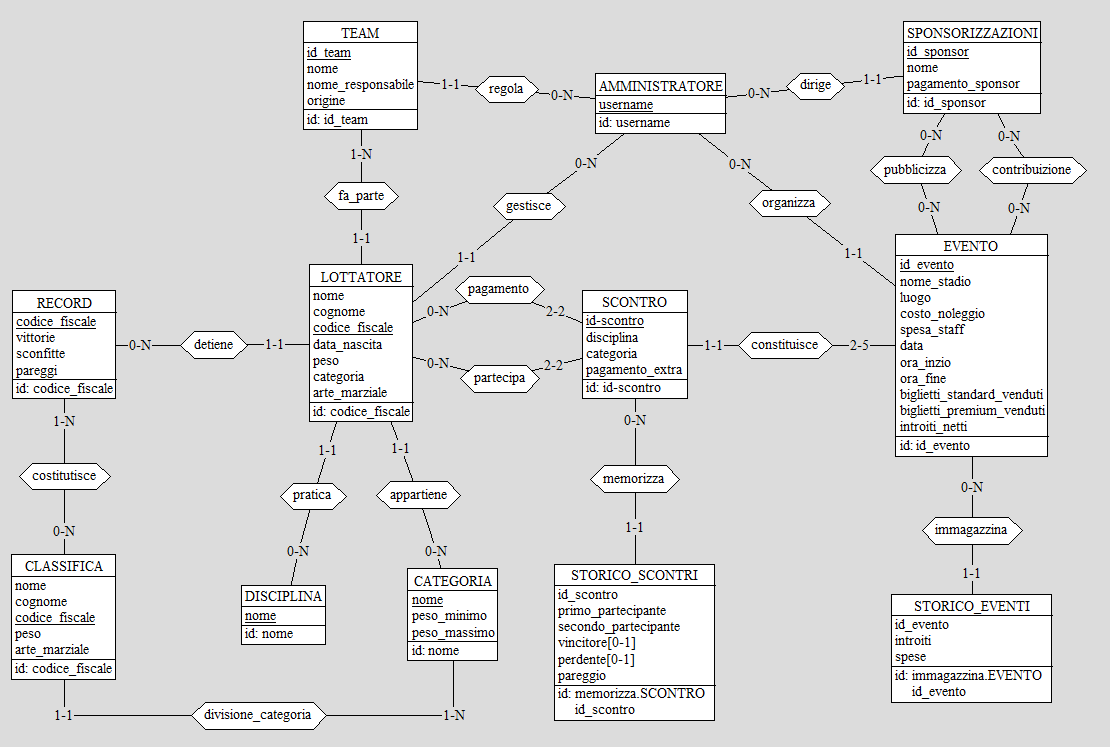
\includegraphics[scale=0.65, angle=90]{./img/schema_finale.png}

\chapter{Progettazione logica}
\section{Stima del volume dei dati}
\begin{itemize}
    \item UTENTE: E, 150
    \item AMMINISTRATORE: E, 1
    \item PUBBLICITARIO: E, 15
    \item crea: A, 1000
    \item NEWS: E, 1000
    \item LOTTATORE: E, 250
    \item CATEGORIA: E, 4
    \item STORICO\textunderscore CATEGORIE: E, 400
    \item pratica: A, 400
    \item contiene: A, 400
    \item STORICO\textunderscore DISCIPLINE: E, 400
    \item appartiene: A, 400
    \item presente: A, 400
    \item DISCIPLINA: E, 3
    \item SCONTRO: E, 2000
    \item tipo: A, 2000
    \item modalità: A, 2000
    \item partecipa: A, 4000
    \item EVENTO: E, 700
    \item constituisce: A, 2000
    \item SPONSORIZZAZIONI: E, 15
    \item sponsorizza: A, 1400
    \item TEAM: E, 150
    \item fa\textunderscore parte: A, 150
\end{itemize}

\section{Descrizione delle operazioni principali e stima della loro frequenza}
\begin{itemize}
    \item Nuovo utente: 1/10 g
    \item Registrazione nuovo lottatore: 1/10 g
    \item Rimuovere un lottatore: 1/15 g
    \item Registrazione nuovo team: 1/12 g
    \item Rimuovere un team: 1/18 g
    \item Registrare un nuovo sponsor: 1/120 g
    \item Rimuovere uno sponsor: 1/210 g
    \item Registrare un evento: 1/20 g
    \item Scrivere news: 1/ g
    \item Rimuovere news: 1/20 g
    \item Registrare pubblicitario: 1/60 g
    \item Rimuovere pubblicitario: 1/90 g
    \item Visualizzare la classifica: 50/ g
    \item Visualizzare lottatori: 30/ g
    \item Visualizzare news: 100/ g
    \item Visualizzare eventi passati: 10/ g
    \item Modificare dati di un partecipante: 1/5 g
\end{itemize} 

\section{Schemi di navigazione e tabelle degli accessi}
\subsection{Registrazione nuovo lottatore}
\begin{table}[H]
    \paragraph{Tavola degli accessi\newline}
    \begin{tabular}{|c|c|c|c|}
    \hline
    Concetto                            & Costrutto & Accessi & Tipo \\ \hline
    LOTTATORE                           & E         & 1       & S    \\ \hline
    TEAM                                & E         & 1       & L    \\ \hline
    DISCIPLINA                          & E         & 1       & L    \\ \hline
    CATEGORIA                           & E         & 1       & L    \\ \hline
    STORICO\textunderscore CATEGORIE    & E         & 2       & S    \\ \hline
    STORICO\textunderscore DISCIPLINE   & E         & 2       & S    \\ \hline
    fa\textunderscore parte             & A         & 1       & L    \\ \hline
    pratica                             & A         & 1       & S    \\ \hline
    contiene                            & A         & 1       & S    \\ \hline
    appartiene                          & A         & 1       & S    \\ \hline
    presente                            & A         & 1       & S    \\ \hline
    \textit{TOTALE}                     &           & 18      &      \\ \hline
    \end{tabular}
\end{table}

\subsection{Rimuovere un lottatore}
\begin{table}[H]
    \paragraph{Tavola degli accessi\newline}
    \begin{tabular}{|c|c|c|c|}
    \hline
    Concetto                            & Costrutto & Accessi & Tipo \\ \hline
    LOTTATORE                           & E         & 1       & S    \\ \hline
    STORICO\textunderscore CATEGORIE    & E         & 1       & S    \\ \hline
    STORICO\textunderscore DISCIPLINE   & E         & 1       & S    \\ \hline
    appartiene                          & A         & 1       & L    \\ \hline
    pratica                             & A         & 1       & L    \\ \hline
    \textit{TOTALE}                     &           & 8       &      \\ \hline
    \end{tabular}
\end{table}

\subsection{Registrazione/Rimozione nuovo team}
\begin{table}[H]
    \paragraph{Tavola degli accessi\newline}
    \begin{tabular}{|c|c|c|c|}
    \hline
    Concetto          & Costrutto & Accessi & Tipo \\ \hline
    TEAM              & E         & 1       & S    \\ \hline
    \textit{TOTALE}   &           & 2       &      \\ \hline
    \end{tabular}
\end{table}

\subsection{Registrare/Rimuovere un nuovo sponsor}
\begin{table}[H]
    \paragraph{Tavola degli accessi\newline}
    \begin{tabular}{|c|c|c|c|}
    \hline
    Concetto          & Costrutto & Accessi & Tipo \\ \hline
    SPONSORIZZAZIONI  & E         & 1       & S    \\ \hline
    \textit{TOTALE}   &           & 2       &      \\ \hline
    \end{tabular}
\end{table}

\subsection{Registrare un evento}
\begin{table}[H]
    \paragraph{Tavola degli accessi\newline}
    \begin{tabular}{|c|c|c|c|}
    \hline
    Concetto                         & Costrutto & Accessi & Tipo \\ \hline
    EVENTO                           & E         & 1       & S    \\ \hline
    SCONTRO                          & E         & 3       & S    \\ \hline
    SPONSORIZZAZIONI                 & E         & 2       & L    \\ \hline
    LOTTATORE                        & E         & 6       & L    \\ \hline
    STORICO\textunderscore CATEGORIE & E         & 6       & L    \\ \hline
    LOTTATORE                        & E         & 6       & S    \\ \hline
    CATEGORIA                        & E         & 6       & L    \\ \hline
    sponsorizza                      & A         & 2       & L    \\ \hline
    partecipa                        & A         & 6       & S    \\ \hline
    constituisce                     & A         & 3       & S    \\ \hline
    tipo                             & A         & 3       & L    \\ \hline
    modalità                         & A         & 3       & L    \\ \hline
    appartiene                       & A         & 6       & L    \\ \hline
    \textit{TOTALE}                  &           & 72      &      \\ \hline
    \end{tabular}
\end{table}

\subsection{Srivere news}
\begin{table}[H]
    \paragraph{Tavola degli accessi\newline}
    \begin{tabular}{|c|c|c|c|}
    \hline
    Concetto          & Costrutto & Accessi & Tipo \\ \hline
    PUBBLICITARIO     & E         & 1       & L    \\ \hline
    NEWS              & E         & 1       & S    \\ \hline
    crea              & A         & 1       & L    \\ \hline
    \textit{TOTALE}   &           & 4       &      \\ \hline
    \end{tabular}
\end{table}

\subsection{Registrare/Rimuovere pubblicitario}
\begin{table}[H]
    \paragraph{Tavola degli accessi\newline}
    \begin{tabular}{|c|c|c|c|}
    \hline
    Concetto          & Costrutto & Accessi & Tipo \\ \hline
    PUBBLICITARIO     & E         & 1       & S    \\ \hline
    \textit{TOTALE}   &           & 2       &      \\ \hline
    \end{tabular}
\end{table}


\subsection{Visualizzare la classifica}
\begin{table}[H]
    \paragraph{Tavola degli accessi\newline}
    \begin{tabular}{|c|c|c|c|}
    \hline
    Concetto                             & Costrutto & Accessi & Tipo \\ \hline
    LOTTATORE                            & E         & 250     & L    \\ \hline
    STORICO\textunderscore CATEGORIE     & E         & 250     & L    \\ \hline
    appartiene                           & A         & 250     & L    \\ \hline
    \textit{TOTALE}                      &           & 750     &      \\ \hline
    \end{tabular}
\end{table}

\subsection{Visualizzare lottatori}
\begin{table}[H]
    \paragraph{Tavola degli accessi\newline}
    \begin{tabular}{|c|c|c|c|}
    \hline
    Concetto                             & Costrutto & Accessi & Tipo \\ \hline
    LOTTATORE                            & E         & 250     & L    \\ \hline
    STORICO\textunderscore CATEGORIE     & E         & 400     & L    \\ \hline
    STORICO\textunderscore DISCIPLINE    & E         & 400     & L    \\ \hline
    TEAM                                 & E         & 150     & L    \\ \hline
    appartiene                           & A         & 400     & L    \\ \hline
    pratica                              & A         & 400     & L    \\ \hline
    fa\textunderscore parte              & A         & 150     & L    \\ \hline
    \textit{TOTALE}                      &           & 2150    &      \\ \hline
    \end{tabular}
\end{table}

\subsection{Visualizzare news}
\begin{table}[H]
    \paragraph{Tavola degli accessi\newline}
    \begin{tabular}{|c|c|c|c|}
    \hline
    Concetto          & Costrutto & Accessi & Tipo \\ \hline
    PUBBLICITARIO     & E         & 15      & L    \\ \hline
    NEWS              & E         & 1000    & L    \\ \hline
    crea              & E         & 1000    & L    \\ \hline
    \textit{TOTALE}   &           & 2015    &      \\ \hline
    \end{tabular}
\end{table}

\subsection{Visualizzare eventi}
\begin{table}[H]
    \paragraph{Tavola degli accessi\newline}
    \begin{tabular}{|c|c|c|c|}
    \hline
    Concetto                    & Costrutto & Accessi & Tipo \\ \hline
    EVENTO                      & E         & 700     & L    \\ \hline
    SPONSORIZZAZIONI            & E         & 1400    & L    \\ \hline
    SCONTRO                     & E         & 2000    & L    \\ \hline
    sponsorizza                 & A         & 1400    & L    \\ \hline
    constituisce                & A         & 400     & L    \\ \hline
    \textit{TOTALE}             &           & 5800    &      \\ \hline
    \end{tabular}
\end{table}


\subsection{Modificare dati di un partecipante}
\begin{table}[H]
    \paragraph{Tavola degli accessi\newline}
    \begin{tabular}{|c|c|c|c|}
    \hline
    Concetto                           & Costrutto & Accessi & Tipo \\ \hline
    LOTTATORE                          & E         & 1       & S    \\ \hline
    STORICO\textunderscore CATEGORIE   & E         & 1       & S    \\ \hline
    STORICO\textunderscore DISCIPLINE  & E         & 1       & S    \\ \hline
    TEAM                               & E         & 1       & L    \\ \hline
    DISCIPLINA                         & E         & 1       & L    \\ \hline
    CATEGORIA                          & E         & 1       & L    \\ \hline
    fa\textunderscore parte            & A         & 1       & L    \\ \hline
    pratica                            & A         & 1       & S    \\ \hline
    contiene                           & A         & 1       & S    \\ \hline
    appartiene                         & A         & 1       & S    \\ \hline
    presente                           & A         & 1       & S    \\ \hline
    \textit{TOTALE}                    &           & 18      &      \\ \hline
    \end{tabular}
\end{table}

\section{Analisi delle ridondanze}
\subsection{Attributo "record" all'interno di "LOTTATORE"}
L'attributo record presente nell'entità lottatore potrebbe essere ricavato attraverso una ricerca di tutte le vittorie, sconfitte 
e pareggi effettuati da un lottatore attraverso l'entità scontro durante la creazione delle classifiche.
\subsubsection{Caso senza ridondanza}
\begin{table}[H]
    \paragraph{Tavola degli accessi creazione classifiche\newline}
    \begin{tabular}{|c|c|c|c|}
    \hline
    Concetto                           & Costrutto & Accessi & Tipo \\ \hline
    LOTTATORE                          & E         & 250     & L    \\ \hline
    SCONTRO                            & E         & 2000    & L    \\ \hline
    STORICO\textunderscore CATEGORIE   & E         & 250     & L    \\ \hline
    partecipa                          & A         & 2000    & L    \\ \hline
    appartiene                         & A         & 250     & L    \\ \hline
    \textit{TOTALE}                    &           & 4750    &      \\ \hline
    \end{tabular}
\end{table}

\begin{table}[H]
    \paragraph{Tavola degli accessi visualizzazione lottatori\newline}
    \begin{tabular}{|c|c|c|c|}
    \hline
    Concetto                           & Costrutto & Accessi & Tipo \\ \hline
    LOTTATORE                          & E         & 250     & L    \\ \hline
    SCONTRO                            & E         & 2000    & L    \\ \hline
    STORICO\textunderscore DISCIPLINE  & E         & 250     & L    \\ \hline
    STORICO\textunderscore CATEGORIE   & E         & 250     & L    \\ \hline
    partecipa                          & A         & 2000    & L    \\ \hline
    pratica                            & A         & 250     & L    \\ \hline
    appartiene                         & A         & 250     & L    \\ \hline
    \textit{TOTALE}                    &           & 5250    &      \\ \hline
    \end{tabular}
\end{table}
\begin{equation}
    \frac{80}{g} \times 10000R = 800000 \frac{R}{g}
\end{equation}

\subsubsection{Caso con ridondanza creazione classifiche}
\begin{table}[H]
    \paragraph{Tavola degli accessi\newline}
    \begin{tabular}{|c|c|c|c|}
    \hline
    Concetto                           & Costrutto & Accessi & Tipo \\ \hline
    LOTTATORE                          & E         & 250     & L    \\ \hline
    STORICO\textunderscore CATEGORIE   & E         & 250     & L    \\ \hline
    appartiene                         & A         & 250     & L    \\ \hline
    \textit{TOTALE}                    &           & 750     &      \\ \hline
    \end{tabular}
\end{table}

\begin{table}[H]
    \paragraph{Tavola degli accessi visualizzazione lottatori\newline}
    \begin{tabular}{|c|c|c|c|}
    \hline
    Concetto                           & Costrutto & Accessi & Tipo \\ \hline
    LOTTATORE                          & E         & 250     & L    \\ \hline
    STORICO\textunderscore DISCIPLINE  & E         & 250     & L    \\ \hline
    STORICO\textunderscore CATEGORIE   & E         & 250     & L    \\ \hline
    pratica                            & A         & 250     & L    \\ \hline
    appartiene                         & A         & 250     & L    \\ \hline
    \textit{TOTALE}                    &           & 1250    &      \\ \hline
    \end{tabular}
\end{table}
\begin{equation}
    \frac{80}{g} \times 2000R = 160000 \frac{R}{g}
\end{equation}
Concludo quindi che devo preservare la ridondanza.

\section{Traduzione di entità e associazioni in relazioni}

Lottatore(\underline{codice\textunderscore fiscale}, nome, cognome, 
data\textunderscore nascita, peso, id\textunderscore team*) $\\$
fk: id\textunderscore team references Team $\\$
$\\$
Team(\underline{id\textunderscore team}, nome, nome\textunderscore responsabile, origine) $\\$
$\\$
Utente(\underline{Username}, pubblicitario*, amministratore*) $\\$
$\\$
News(\underline{id\textunderscore news}, argomento, descrizione, Username) $\\$
fk: Username references Pubblicitario $\\$
$\\$
Sponsorizzazioni(\underline{id\textunderscore sponsor}, nome, pagamento\textunderscore sponsor) $\\$
$\\$
Evento(\underline{id\textunderscore evento}, nome\textunderscore stadio, 
luogo, costo\textunderscore noleggio, spesa\textunderscore staff, data, ora\textunderscore inizio, ora\textunderscore fine, 
sponsor1*, sponsor2*, sponsor3*, introiti, spese, biglietti\textunderscore standard\textunderscore venduti, 
biglietti\textunderscore premium\textunderscore venduti, 
costo\textunderscore biglietti\textunderscore standard, costo\textunderscore biglietti\textunderscore premium) $\\$
fk: sponsor references Sponsorizzazioni $\\$
$\\$
Scontro(\underline{id\textunderscore scontro, id\textunderscore evento}, pareggio, disciplina, categoria, pagamento\textunderscore extra) $\\$
fk: id\textunderscore evento references Evento $\\$
fk: categoria references Categoria $\\$
fk: disciplina references Disciplina $\\$
$\\$
Partecipa(\underline{id\textunderscore scontro, id\textunderscore evento, codice\textunderscore fiscale}, vincitore) $\\$
fk: (id\textunderscore evento, id\textunderscore scontro) references Scontro $\\$
fk: codice\textunderscore fiscale references Lottatore $\\$
$\\$
Categoria(\underline{nome}, peso\textunderscore minimo, peso\textunderscore massimo) $\\$
$\\$
Storico\textunderscore Categorie(\underline{codice\textunderscore fiscale, periodo}, nome\textunderscore cat) $\\$
fk: codice\textunderscore fiscale references Lottatore $\\$
fk: nome\textunderscore cat references Categoria $\\$
$\\$
Disciplina(\underline{nome}) $\\$
$\\$
Storico\textunderscore Discipline(\underline{codice\textunderscore fiscale, periodo}, nome\textunderscore disc) $\\$
fk: codice\textunderscore fiscale references Lottatore $\\$
fk: nome\textunderscore disc references Disciplina $\\$

\section{Schema relazionale finale}
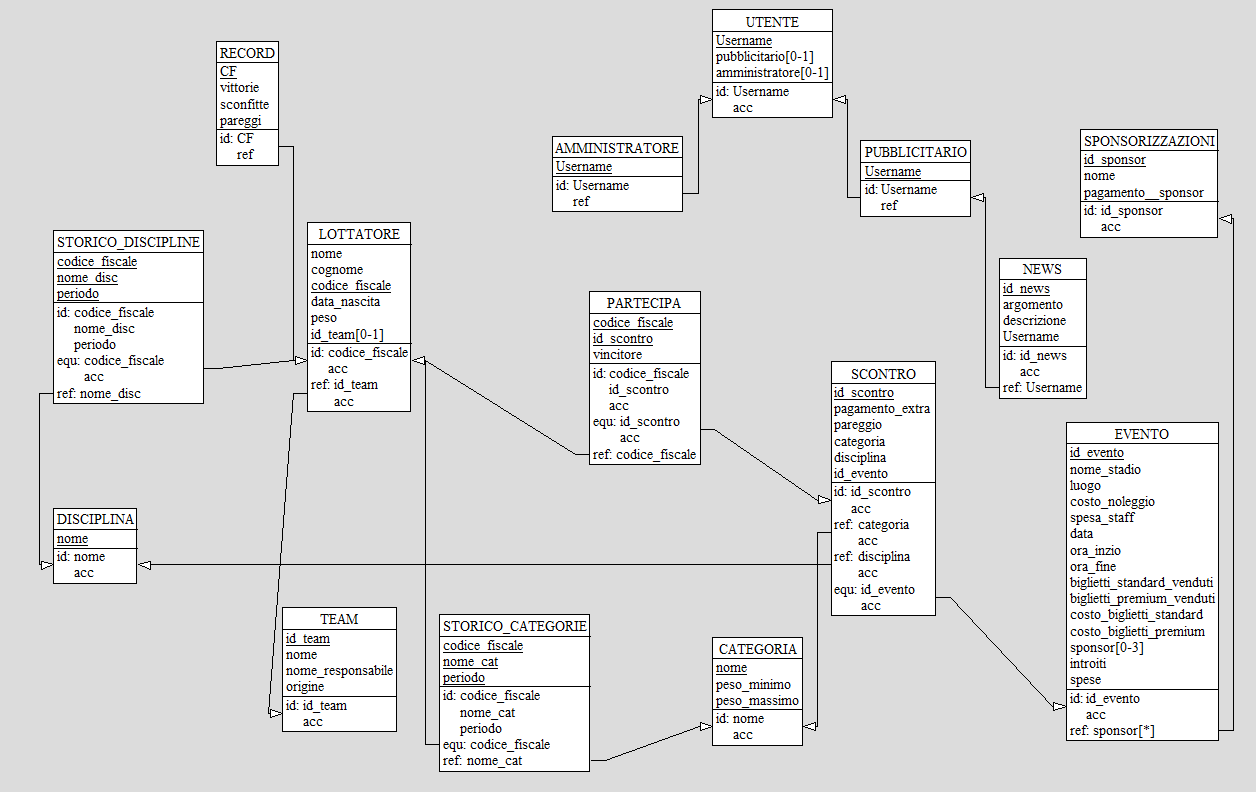
\includegraphics[scale=0.65, angle=90]{./img/schema_rel_finale.png}

\section{Traduzione operazioni in query SQL}
\subsection{Creazione tabelle}
\begin{verbatim}
CREATE TABLE UTENTE (
    username varchar(40) NOT NULL,
    passw varchar(40) NOT NULL,
    tipo varchar(30) NOT NULL,
    PRIMARY KEY (username)
);

CREATE TABLE LOTTATORE (
    codiceFiscale varchar(50) NOT NULL,
    nome varchar(20) NOT NULL,
    cognome varchar(30) NOT NULL,
    dataNascita date NOT NULL,
    peso float NOT NULL,
    id_team integer,
    vittorie number NOT NULL,
    sconfitte number NOT NULL,
    pareggi number NOT NULL,
    PRIMARY KEY (codiceFiscale),
    CONSTRAINT (id_team) SET NULL ON DELETE
);

CREATE TABLE TEAM (
    idTeam integer NOT NULL,
    nome varchar(50) NOT NULL,
    nome_responsabile varchar(20),
    origine varchar(40),
    PRIMARY KEY (idTeam)
);

CREATE TABLE DISCIPLINA (
    nome ENUM('BJJ','MMA','MuayThai') PRIMARY KEY
);

CREATE TABLE STORICO_DISCIPLINE (
    codiceFiscale varchar(50) NOT NULL,
    nome_disc varchar(16) NOT NULL,
    periodo varchar(32) NOT NULL,
    PRIMARY KEY (codiceFiscale, periodo)
);

CREATE TABLE CATEGORIA (
    nome ENUM('PesoPiuma','Welterweight',
            'PesoMedio','PesiMassimi') PRIMARY KEY,
    pesoMinimo integer,
    pesiMassimi integer 
);

CREATE TABLE STORICO_CATEGORIE (
    codiceFiscale varchar(50) NOT NULL,
    nome_cat varchar(16) NOT NULL,
    periodo varchar(32) NOT NULL,
    PRIMARY KEY (codiceFiscale, periodo)
);

CREATE TABLE PARTECIPA (
    codiceFiscale varchar(50) NOT NULL,
    idScontro integer NOT NULL,
    idEvento integer NOT NULL,
    vincitore varchar(50),
    PRIMARY KEY (codiceFiscale, idScontro, idEVento)
);

CREATE TABLE SCONTRO (
    idEvento integer NOT NULL,
    idScontro integer NOT NULL,
    disciplina ENUM('BJJ','MMA','MuayThai'),
    categoria ENUM('PesoPiuma','Welterweight',
                    'PesoMedio','PesiMassimi'),
    pagamentoExtra float,
    pareggio bool,
    PRIMARY KEY (idEvento, idScontro)
);

CREATE TABLE EVENTO (
    idEvento integer NOT NULL,
    nomeStadio varchar(40) NOT NULL,
    luogo varchar (50) NOT NULL,
    costoNoleggio float,
    spesaStaff float,
    dataEvento date NOT NULL,
    oraInizio varchar(10) NOT NULL,
    oraFine varchar(10) NOT NULL,
    bigliettiStandardVenduti integer,
    bigliettiPremiumVenduti integer,
    costoBigliettiPremium integer,
    costoBigliettiStandard integer,
    sponsor JSON,
    introiti float,
    spese float,
    PRIMARY KEY (idEvento)
    CONSTRAINT ORARIO CHECK (oraInizio <= oraFine) => 
        (Rimosso perchè risultava esserci un 
        problema quando gli eventi 
        finivano dopo mezzanotte)
);

CREATE TABLE SPONSORIZZAZIONI (
    idSponsor integer NOT NULL,
    nome varchar(40) NOT NULL,
    pagamentoSponsor float,
    PRIMARY KEY (idSponsor)
);

CREATE TABLE NEWS (
    idNews integer NOT NULL,
    argomento varchar(128) NOT NULL,
    descrizione varchar(4096) NOT NULL,
    scrittore varchar(40) NOT NULL,
    PRIMARY KEY (idNews)
);

\end{verbatim}
\subsection{Operazioni amministratore}
\subsubsection{Aggiungere lottatore}
\begin{verbatim}
INSERT INTO LOTTATORE (nome, cognome, codiceFiscale, 
    dataNascita, id_team, peso, vittorie, sconfitte, pareggi)
VALUES (?, ?, ?, ?, ?, ?, 0, 0, 0);

--inserisco inoltre CF, categoria e disciplina negli storici--

INSERT INTO STORICO_CATEGORIE (codiceFiscale, categoria)
VALUES (?, ?, "ongoing");

INSERT INTO STORICO_DISCIPLINE (codiceFiscale, disciplina)
VALUES (?, ?, "ongoing");


\end{verbatim}
\subsubsection{Rimuovere lottatore}
\begin{verbatim}
DELETE FROM LOTTATORE
WHERE codiceFiscale = ?;

-- Elimina da storico_categoria e storico_disciplina --

DELTE FROM STORICO_DISCIPLINE
WHERE codiceFiscale = ?;

DELTE FROM STORICO_CATEGORIE
WHERE codiceFiscale = ?;

\end{verbatim}
\subsubsection{Aggiungere team}
\begin{verbatim}
INSERT INTO TEAM (idTeam, nome, nome_responsabile, origine)
VALUES(?, ?, ?, ?);
\end{verbatim}
\subsubsection{Rimuovere team}
\begin{verbatim}
DELETE FROM TEAM 
WHERE idTeam = ?

-- si rimuove l'attributo da tutti i lottatori che fanno 
parte di questo team --
UPDATE LOTTATORE
SET id_team= NULL
WHERE id_team = ?
\end{verbatim}
\subsubsection{Aggiungere sponsor}
\begin{verbatim}
INSERT INTO SPONSORIZZAZIONI(idSponsor, nome, pagamentoSponsor)
VALUES (?, ?, ?);
\end{verbatim}
\subsubsection{Rimuovere sponsor}
\begin{verbatim}
DELETE FROM SPONSORIZZAZIONI
WHERE idSponsor = ?
\end{verbatim}
\subsubsection{Scrivere news}
\begin{verbatim}
INSERT INTO UTENTE(idNews, argomento, descrizione, scrittore)
VALUES (?, ?, ?, ?);
\end{verbatim}
\subsubsection{Rimuovere news}
\begin{verbatim}
DELETE FROM NEWS
WHERE id_news = ?
\end{verbatim}
\subsubsection{Aggiungere Pubblicitario/Utente}
\begin{verbatim}
INSERT INTO UTENTE(username, passw, tipo)
VALUES (?, ?, ?);
\end{verbatim}
\subsubsection{Rimuovere pubblicitario}
\begin{verbatim}
DELETE FROM UTENTE
WHERE Username = ?
\end{verbatim}
\subsubsection{Registrare evento}
\begin{verbatim}
INSERT INTO EVENTO (idEVento, nomeStadio, luogo, costoNoleggio,
    spesaStaff, dataEvento, oraInizio, oraFine, 
    bigliettiStandardVenduti, bigliettiPremiumVenduti, 
    costoBigliettiStandard, costoBigliettiPremium, sponsor, 
    introiti, spese, guadagnoComplessivo)
VALUES (?, ?, ?, ?, ?, ?, ?, ?, ?, ?, ?, ?, 
        ?, ?, ?, introiti - spese);

-- Aggiungere Scontro (2-5 volte, in base al tipo di evento) --

INSERT INTO SCONTRO (idEvento, idScontro, disciplina, 
    categoria, pagamentoExtra, pareggio)
VALUES (?, ?, ?, ?, ?, ?);

INSERT INTO PARTECIPA (id_evnto, codice_fiscale, id_scontro, 
    vincitore)
VALUES (?, ?, ?, ?)

UPDATE LOTTATORE
SET vittorie = ?, sconfitte = ?, pareggi = ?
WHERE codiceFiscale = ?

\end{verbatim}
\subsubsection{Modificare lottatore}
\begin{verbatim}

UPDATE LOTTATORE 
SET nome = ?, cognome = ?,
    dataNascita = ?, id_team = ?, 
    peso = ?, vittorie = ?, sconfitte = ?,
    pareggi = ?
WHERE codiceFiscale = ?

-- controllo se la riga che voglio inserire esiste già, 
e se sì, lascio tutto così come è altrimenti modifico 
questa impostando la data di oggi nel campo periodo e 
inserisco una nuova riga con la nuova disciplina voluta 
e stato "ongoing" --

UPDATE STORICO_DISCIPLINE
SET periodo = ?
WHERE codiceFiscale = ? 
    AND periodo = 'ongoing' AND nome_disc <> ?;

INSERT INTO STORICO_DISCIPLINE 
    (codiceFiscale, nome_disc, periodo)
SELECT ?, ?, 'ongoing'
WHERE NOT EXISTS (
    SELECT 1
    FROM STORICO_DISCIPLINE
    WHERE codiceFiscale = ?
        AND periodo = 'ongoing' AND nome_disc <> ?
);

-- eseguo la stessa cosa per le categorie --

UPDATE STORICO_CATEGORIE
SET periodo = ?
WHERE codiceFiscale = ? 
    AND periodo = 'ongoing' AND nome_disc <> ?;

INSERT INTO STORICO_CATEGORIE 
    (codiceFiscale, nome_disc, periodo)
SELECT ?, ?, 'ongoing'
WHERE NOT EXISTS (
    SELECT 1
    FROM STORICO_CATEGORIE
    WHERE codiceFiscale = ?
        AND periodo = 'ongoing' AND nome_disc <> ?
);
    
\end{verbatim}
\subsubsection{Visualizzare news}
\begin{verbatim}
SELECT *
FROM NEWS
\end{verbatim}
\subsubsection{Visualizzare lottatore}
\begin{verbatim}
SELECT *
FROM LOTTATORE l
LEFT JOIN STORICO_CATEGORIE sc ON 
    l.codiceFiscale = sc.codiceFiscale
LEFT JOIN STORICO_DISCIPLINE sd ON 
    l.codiceFiscale = sd.codiceFiscale
ORDER BY l.codiceFiscale;    
\end{verbatim}
\subsubsection{Visualizzare eventi}
\begin{verbatim}
SELECT *
FROM EVENTO e
LEFT JOIN SCONTRO s ON e.idEvento = s.idEvento
ORDER BY e.idEvento, s.idScontro;
\end{verbatim}
\subsubsection{Visualizzare classifiche}
\begin{verbatim}
SELECT *
FROM LOTTATORE l
INNER JOIN STORICO_DISCIPLINE s
    ON l.codiceFiscale = s.codiceFiscale
    WHERE s.periodo = "ongoing" AND s.nome_disc = ?;
\end{verbatim}

\chapter{Progettazione dell'applicazione}
\section{Descrizione dell'architettura dell'applicazione realizzata}
L'applicazione che permette di gestire il database è stata creata utilizzando \textrm{Typescript} in combinazione con il framework 
\emph{React}, mentre per quanto riguarda il database, esso risiede in locale ed è stato sviluppato usando \emph{MySQL}.
L'applicazione è un'applicazione web che si appoggia a un server locale. Essa consente quindi la possibilità di connettere 
frontend e backend utilizzando il protocollo \textbf{HTTP}, e quindi attraverso delle \textbf{API REST}. Grazie a un server locale, 
il backend avrà la possibilità di ricevere richieste dal frontend, portando con sé parametri e restituendo valori, il tutto 
evitando una connessione diretta tramite codice. Questo design permette all'applicazione di avere una scalabilità maggiore, eliminando 
eventuali dipendenze tra frontend e backend. Inoltre, per la gestione del database da parte del backend, si utilizza la libreria 
\emph{TypeORM} di \textrm{Typescript}. Libreria che permette di eseguire operazioni sui dati mediante codice.


\begin{figure}
    \centering
    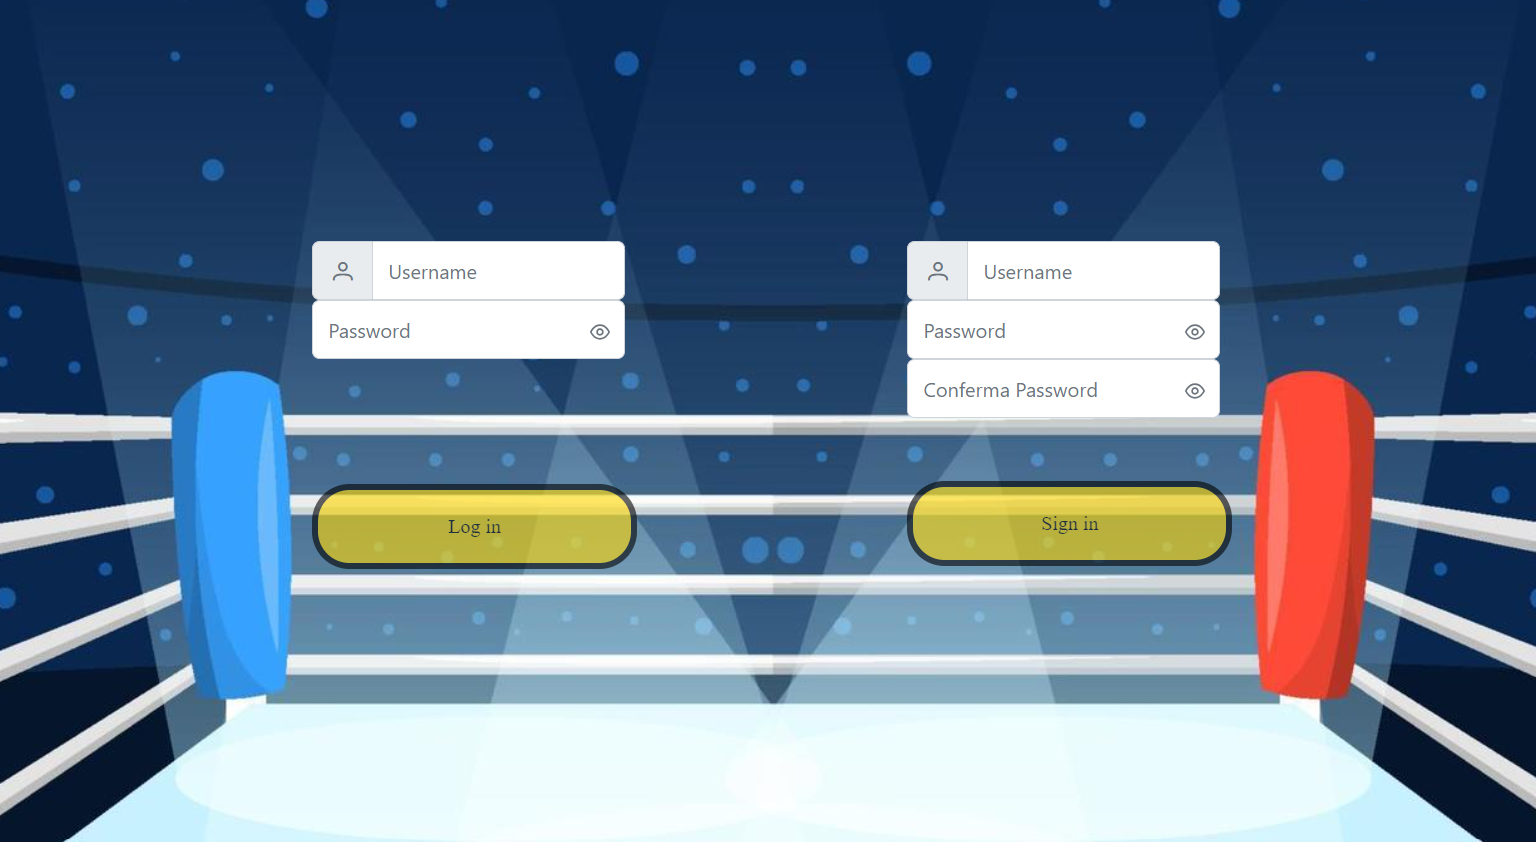
\includegraphics[scale=0.4]{./img/login.png}
    \caption{\textit{log in/sign in}}
    \medskip
    Da questa pagina (iniziale) è possibile accedere in 3 diverse maniere (amministratore, pubblicitario, utente), ognuna
    di queste darà accesso a diverse operazioni cambiando anche le interfacce.
\end{figure}

\begin{figure}
    \centering
    \includegraphics[scale=0.3]{./img/menù_iniziale.png}
    \caption{\textit{Menù iniziale dell'applicazione}}
    \medskip
    In questo menù accessibile solo dall'amministratore sarà possibile accedere alle operazioni di gestione del 
    database(es: \ref{addEvento} per la registrazione di un evento) oppure alle classifiche generali dei lottatori \ref{categoria}.
\end{figure}

\begin{figure}
    \centering
    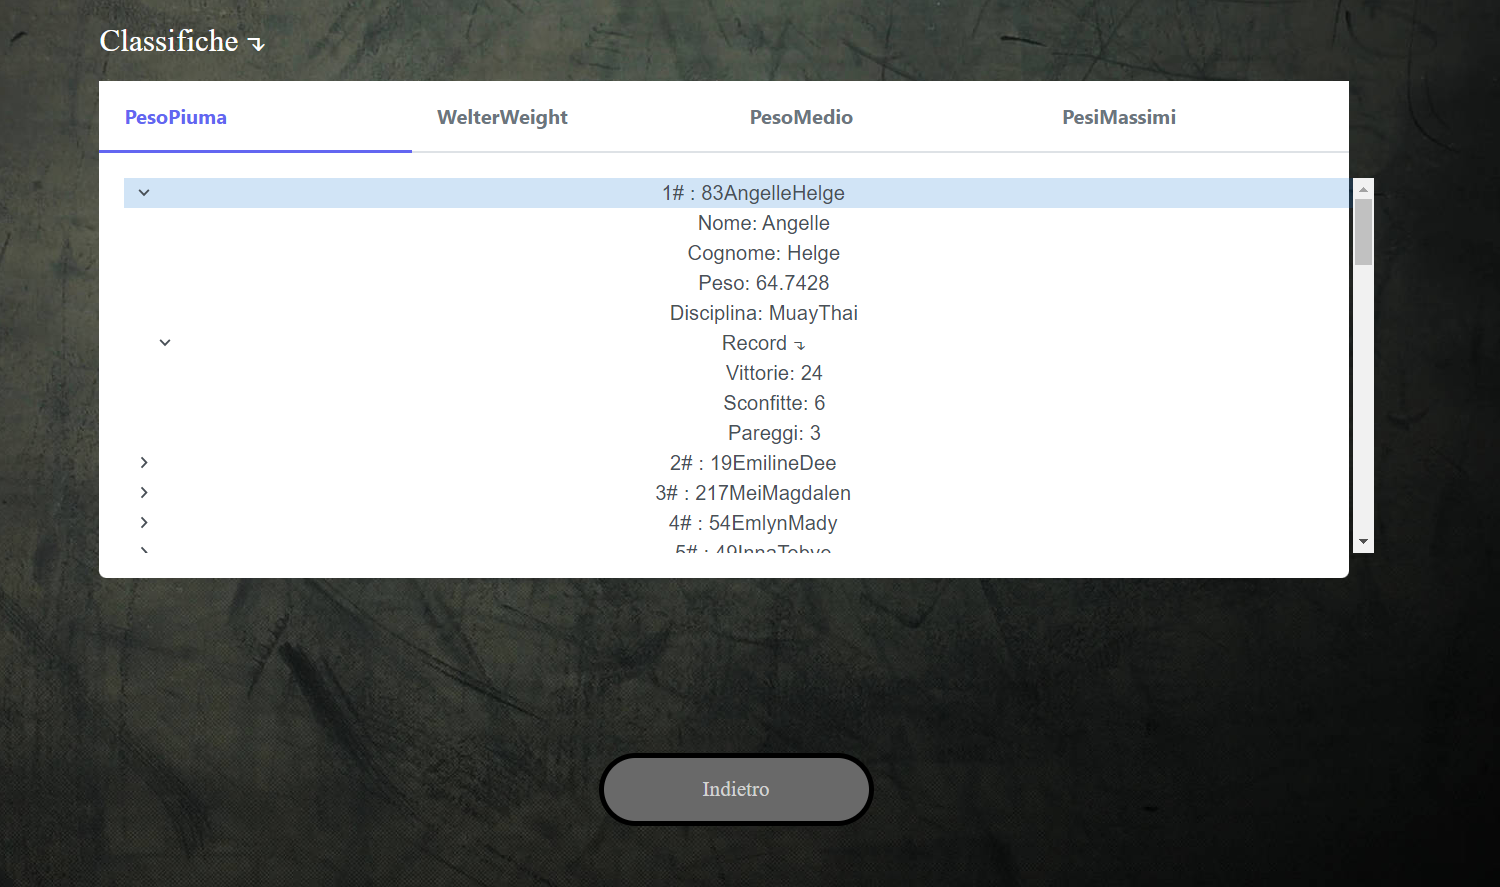
\includegraphics[scale=0.4]{./img/classifiche.png}
    \caption{\textit{Classifiche di tutti i partecipanti divisi in categorie}}
    \label{categoria}
\end{figure}

\begin{figure}
    \centering
    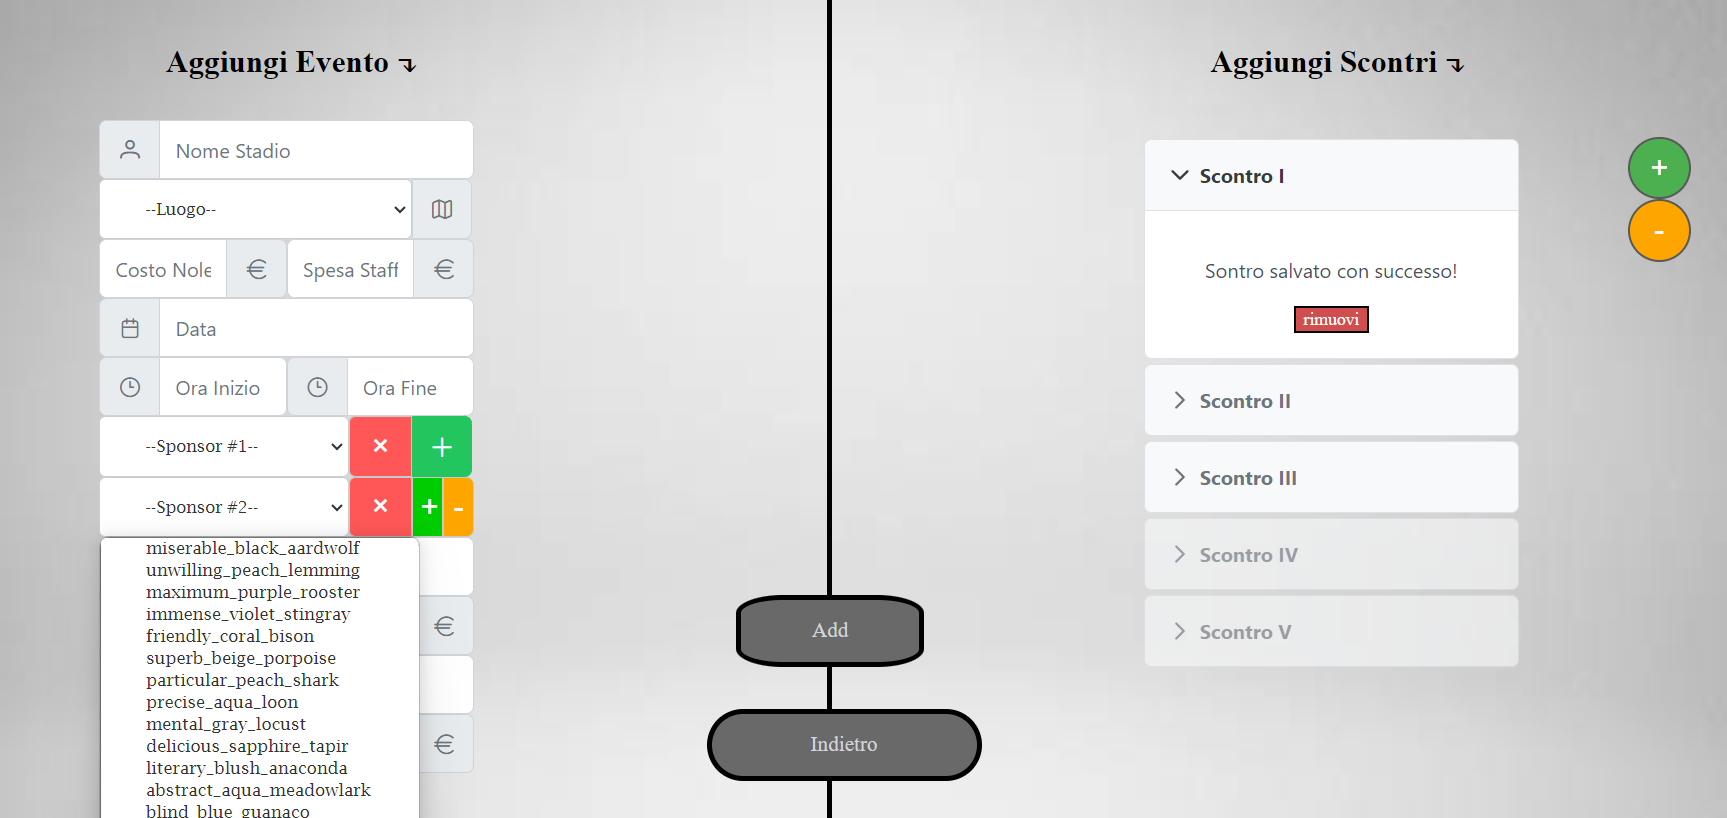
\includegraphics[scale=0.35]{./img/eventoAdd.png}
    \caption{\textit{Pagina che permette di registrare un evento e i proprio scontri}}
    \medskip
    Come si puo notare dall'immagine qua abbiamo una schermata dove è possibile registrare Eventi inserendo tutti i dati necessari nella 
    parte sinistra dello schermo, nella parte destra invece potremmo aggiungere da 2 a 5 scontri (in questo caso notiamo che 
    uno è già stato aggiunto e ci viene proposta la possibilità di rimuoverlo e modificarlo se desiderato).
    \label{addEvento}
\end{figure}

\begin{figure}
    \centering
    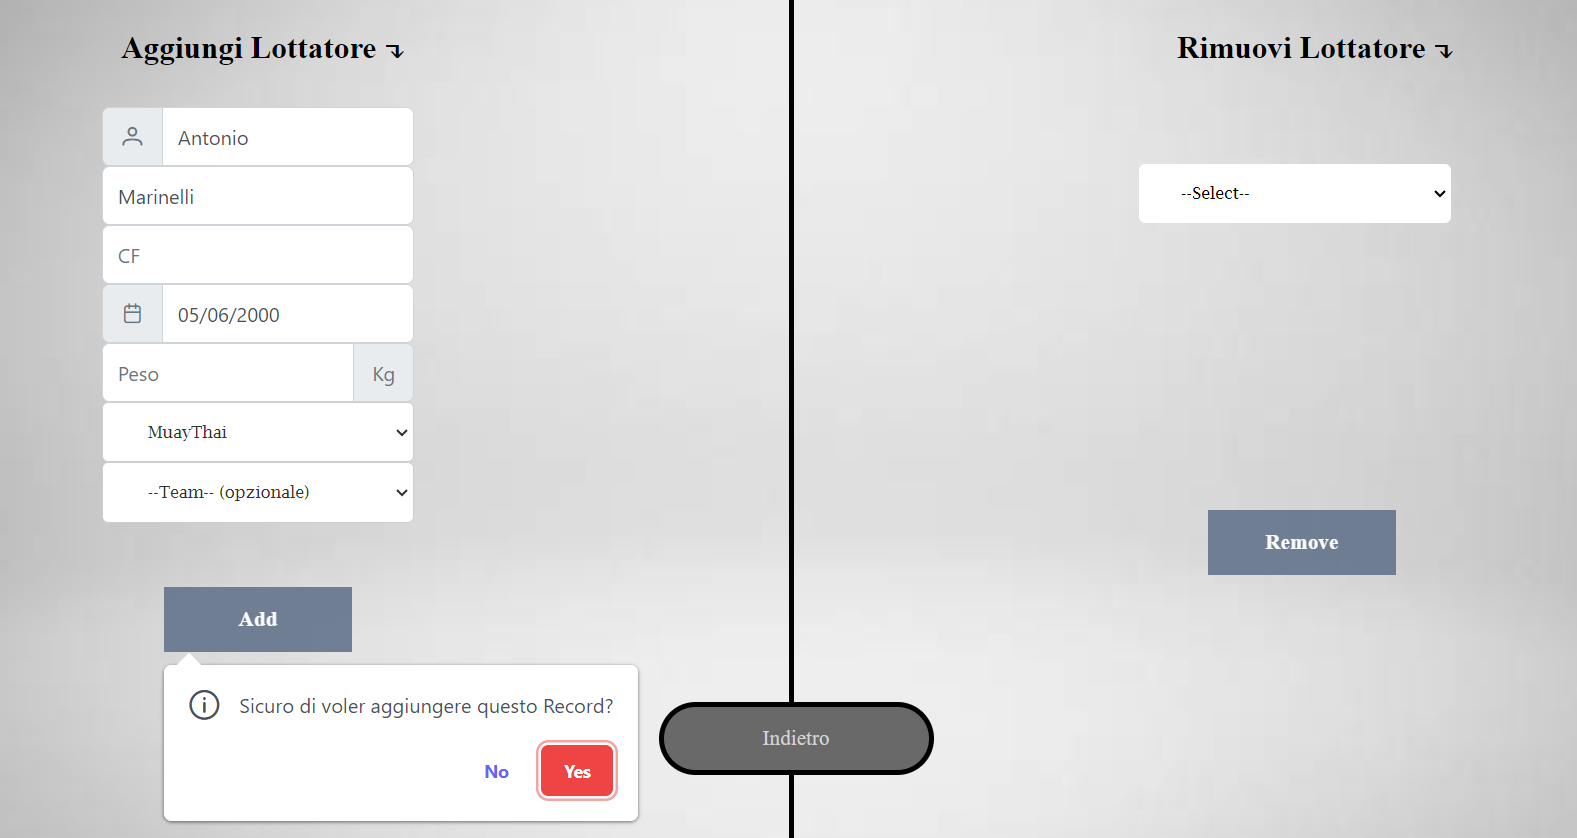
\includegraphics[scale=0.4]{./img/AddLottatore.png}
    \caption{\textit{Pagina che ci permette di aggiungere e rimuovere lottatori}}
\end{figure}



\end{document}
